\documentclass[11pt]{elegantbook}
\definecolor{structurecolor}{RGB}{40,58,129}
\linespread{1.6}
\setlength{\footskip}{20pt}
\setlength{\parindent}{0pt}
\newcommand{\argmax}{\operatornamewithlimits{argmax}}
\newcommand{\argmin}{\operatornamewithlimits{argmin}}
\elegantnewtheorem{proof}{Proof}{}{Proof}
\elegantnewtheorem{claim}{Claim}{prostyle}{Claim}
\DeclareMathOperator{\col}{col}
\title{\textbf{Linear Algebra}}
\author{Wenxiao Yang}
\institute{University of Illinois at Urbana-Champaign; University of California Berkeley}
\date{2023 (Last Updated)}
\setcounter{tocdepth}{2}
\cover{cover.jpg}
\extrainfo{All models are wrong, but some are useful.}

% modify the color in the middle of titlepage
\definecolor{customcolor}{RGB}{32,178,170}
\colorlet{coverlinecolor}{customcolor}
\usepackage{cprotect}

\addbibresource[location=local]{reference.bib} % bib

\begin{document}

\maketitle
\frontmatter
\tableofcontents
\mainmatter


\chapter{Field and Vector Space}
\section{Field $(\mathbb{F},+,\cdot)$}
\subsection{Definition of Field \small{(@ Lec 02 of ECON 204)}}
\begin{definition}[Field]
    \normalfont
    A \textbf{field} $\mathcal{F}=(\mathbb{F},+,\cdot)$ is a 3-tuple consisting of a set $\mathbb{F}$ and two binary operations $+,\cdot: \mathbb{F}\times \mathbb{F} \rightarrow \mathbb{F}$ such that
    \begin{enumerate}
        \item $+$ is associative, commutative.
        \item Exists (unique) additive identity and (unique) additive inverse.
        \item $\cdot$ is associative, commutative.
        \item Exists (unique) multiplicative identity and (unique) multiplicative inverse.
        \item Distributivity of multiplication over addition.
    \end{enumerate}
\end{definition}

\begin{example}[ of Field]
    \begin{enumerate}
        \item $\mathbb{R}$, $\mathbb{C}$, $\mathbb{Q}$ are field;
        \item $\mathbb{N}$, $\mathbb{Z}$ are not field;
        \item $\mathbb{Q}(\sqrt{2})=\{q+r\sqrt{2}: q,r\in \mathbb{Q}\}$ is the smallest filed containing $\mathbb{Q}\cup \sqrt{2}$.
    \end{enumerate}
\end{example}

\section{Vector Space}
\subsection{Definition of Vector Space \small{(@ Lec 02 of ECON 204)}}
\begin{definition}[Vector Space]
    \normalfont
    A \underline{vector space} over a field $\mathbb{F}$, $(V, \mathbb{F}, +,\times)$, is a set $V$ w/ an operation \underline{addition} $+ : V \times V \rightarrow V$ and an operation \underline{scalar multiplication} $\mathbb{F} \times V \rightarrow V$
    \begin{enumerate}
        \item $+$ is associative, commutative.
        \item Exists (unique) additive identity and (unique) additive inverse.
        \item $\cdot$ is associative (there is no need to consider commutativity).
        \item Exists (unique) multiplicative identity (there is no need to consider inverse).
        \item Distributivity of scalar multiplication over vector addition: $\forall \alpha\in\mathbb{F},\ v,u\in V,\ \alpha(v+u)=\alpha v+\alpha u$
        \item Distributivity of scalar multiplication over scalar addition: $\forall \alpha,\beta\in\mathbb{F},\ v\in V,\ (\alpha+\beta)v=\alpha v+\beta v$
    \end{enumerate}
\end{definition}
We often say “$V$ is a vector space over $\mathbb{F}$”.

\begin{example}
    \begin{enumerate}
        \item $\mathbb{R}^n$ is a vector space over $\mathbb{R}$, for any $n\in \mathbb{N}$.
        \item $\mathbb{Q}(\sqrt{2})$ is a vector space over $\mathbb{Q}$. (It is $\mathbb{Q}^2$, using $(q,r)$ versus $q+r\sqrt{2}$).
        \item $\mathbb{Q}(\sqrt[3]{2})$ is a vector space over $\mathbb{Q}$. (It is $\mathbb{Q}^3$, using $(q,r,v)$ versus $q+r 2^\frac{2}{3}+v2^\frac{1}{3}$).
        \item $C([0,1])$, the space of all continuous real-valued functions on $[0,1]$, is a vector space over $\mathbb{R}$.
    \end{enumerate}
\end{example}

\subsection{Theorem: A field is a vector space over its subfield}
\begin{theorem}
    $\mathbb{K}\subset\mathbb{F}$ is a subfield of a field $\mathbb{F}$. Then $\mathbb{F}$ is a vector space over $\mathbb{K}$.
\end{theorem}
\begin{example}
    Since $\mathbb{F}\subset \mathbb{F}[x]$, then $\mathbb{F}[x]$ is a vector space over $\mathbb{F}$.
\end{example}
\subsection{Vector Subspace}
Suppose that $V$ is a vector space over $\mathbb{F}$. A \underline{vector subspace} or just \underline{subspace} is a nonempty subset $W\subset V$ closed under addition and scalar multiplication. i.e. $v+w\in W,\ av\in W,\ \forall v,w\in W,\ a\in \mathbb{F}$.
\begin{example}
$\mathbb{K}\subset \mathbb{L}\subset \mathbb{F}$, then $\mathbb{L}$ is a subspace of $\mathbb{F}$ over $\mathbb{K}$.
\end{example}
\subsection{Linear Independent}
\begin{definition}[Linear Independence]
    \normalfont
    A set $V \subseteq X$ is \textbf{linearly dependent} if there exist $v_1,...,v_n \in V$ and $\alpha_1,...,\alpha_n \in F$ not all zero such that $\sum_{i=1}^n\alpha_iv_i=0$.
\end{definition}
Prove a set is linearly independent by $\sum_{i=1}^n\alpha_iv_i=0 \Rightarrow \alpha_i=0,\forall i$.

\subsection{span V, basis, dimension}
\begin{definition}[Span]
    \normalfont
    If $V \subseteq X$, the span of $V$, denoted $\textnormal{span }V$, is the set of all linear combinations of elements of $V$.
    The set $V \subseteq X$ \textbf{spans} $X$ if $\textnormal{span }V=X$.
\end{definition}

\begin{definition}[(Hamel) Basis]
    \normalfont
    A \textbf{Hamel basis} (often just called a \textbf{basis}) of a vector space $X$ is a \textbf{linearly independent} set of vectors in $X$ that \textbf{spans} $X$.
\end{definition}
\begin{theorem}
    Every vector space has a Hamel basis.
\end{theorem}

\begin{theorem}[Bases have the same cardinality]
    Any two Hamel bases of a vector space $X$ have the same cardinality (are numerically equivalent).
\end{theorem}

\begin{theorem}[Unique Representation]\label{unique}
    Let $V$ be a Hamel basis for $X$. Then every vector $x \in X$ has a \textbf{unique representation} as a linear combination of a finite number of elements of $V$\\(with all coefficients nonzero, unique representation of $0=\sum_{i\in \emptyset}\alpha_i v_i$).
\end{theorem}

\begin{proposition}[Proposition 2.4.10.]
    Suppose $V$ is a vector space over a field $\mathbb{F}$ having a basis $\{v_1,...,v_n\}$ with $n \geq 1$.
    \begin{enumerate}[(i).]
        \item For all $v \in V$, $v = a_1 v_1 +... + a_n v_n$ for exactly one $(a_1,...,a_n)\in \mathbb{F}^n$ (unique representation).
        \item If $w_1,...,w_n$ span $V$, then they are linearly independent.
        \item If $w_1,...,w_n$ are linearly independent, then they span $V$.
    \end{enumerate}
\end{proposition}

\subsection{Dimension}
\begin{definition}[Dimension]
    \normalfont
    The dimension of a vector space $X$, denoted $\dim X$, is the cardinality of any basis of $X$.
\end{definition}
If a vector space $V$ over $\mathbb{F}$ has a basis with $n$ vectors, then $V$ is said to be n-dimensional (over $\mathbb{F}$) or is said to have \textbf{dimension} $n$.
\begin{definition}[Finite-Dimension]
    \normalfont
    Let $X$ be a vector space. If $\dim X = n$ for some $n \in N$, then $X$ is finite-dimensional. Otherwise, $X$ is infinite-dimensional.
\end{definition}

\subsection{Theorem: $|V|>\dim X \Rightarrow$ linearly dependent}
\begin{theorem}[$|V|>\dim X \Rightarrow$ $V$ is linearly dependent]
    Suppose $\dim X = n \in \mathbb{N}$. If $V \subseteq X$ and $|V| > n$, then $V$ is linearly dependent.
\end{theorem}

\subsection{Theorem: $|V|=n$: Linear Indep $\Leftrightarrow$ Spans $\Rightarrow$ Basis}
\begin{theorem}[$|V|=n$: Linear Indep $\Leftrightarrow$ Spans $\Rightarrow$ Basis]
    Suppose $\dim X = n \in \mathbb{N}$, and $V \subseteq X$ and $|V| = n$.
    \begin{enumerate}
        \item If $V$ is linearly independent, then $V$ spans $X$, so $V$ is a Hamel basis.
        \item If $V$ spans $X$, then $V$ is linearly independent, so $V$ is a Hamel basis.
    \end{enumerate}
\end{theorem}





\subsection{Standard basis vectors}
$e_1=(1,0,...,0),e_2=(0,1,0,...,0),...,e_n=(0,0,...,0,1)\in \mathbb{F}^n$ are a basis for $\mathbb{F}^n$ called the \textbf{standard basis vectors}.


\section{Linear Transformation}
\subsection{Definition of Linear Transformation}
\begin{definition}[Linear Transformation]
    \normalfont
    Given two vector spaces $V$ and $W$ over $\mathbb{F}$ a \textbf{linear transformation} is a function $T : V \rightarrow	 W$ such that
for all $a \in \mathbb{F}$ and $v,w \in V$, we have
\begin{equation}
    \begin{aligned}
        T(av)=aT(v) \textnormal{ and } T(v+w)=T(v)+T(w)
    \end{aligned}
    \nonumber
\end{equation}
\end{definition}

\subsection{Composition of Linear Transformations is also Linear}
Let $L(X, Y)$ denote the \textbf{set of all linear transformations} from $X$ to $Y$ over field $\mathbb{F}$.
\begin{theorem}
    $L(X,Y)$ is a vector space of $\mathbb{F}$.
\end{theorem}

\begin{proposition}[Composition of Linear Transformations is also Linear]
    Suppose $R\in L(X,Y),\ S\in L(Y,Z)$, then $S\circ R\in L(X,Z)$.
\end{proposition}

\subsection{Function from a Basis extends uniquely to a Linear Transformation}
\begin{proposition}[Proposition 2.4.15.]
    If $V$ and $W$ are vector spaces and $v_1,...,v_n$ is a basis for $V$ then any function
    from $\{v_1,...,v_n\}\rightarrow W$ extends \textit{uniquely} to a linear transformation $V \rightarrow W$.
\end{proposition}
Any $v\in V$, $\exists (a_1,...,a_n)$ s.t. $v=a_1 v_1+...+a_n v_n$. Then $T(v)=T(a_1 v_1+...+a_n v_n)=a_1T(v_1)+...+a_nT(v_n)$

\subsection{Image, Kernel, Rank}
\begin{definition}[Image, Kernel, Rank]
    \normalfont
    Let $T\in L(X,Y)$,
    \begin{enumerate}[$\circ$]
        \item The \textbf{image} of $T$ is $\textnormal{Im }T= T(X)\subseteq Y$.
        \item The \textbf{kernel} of $T$ is $\textnormal{ker }T=\{x\in X:T(x)=0\}$.
        \item The \textbf{rank} of $T$ is $\textnormal{Rank }T=\dim(\textnormal{Im }T)$.
    \end{enumerate}
\end{definition}


\subsection{The Rank-Nullity Theorem: $\dim X=\dim\textnormal{ker }T+\textnormal{Rank }T$}
\begin{theorem}[The Rank-Nullity Theorem]
    Let $X$ be a finite-dimensional vector space and $T \in L(X, Y)$. Then $\textnormal{Im }T$ and $\textnormal{ker }T$ are vector subspaces of $Y$ and $X$ respectively, and
    $$\dim X=\dim\textnormal{ker }T+\textnormal{Rank }T$$
\end{theorem}


\subsection{Theorem: Linear Transformation $T$ is 1-to-1 $\Leftrightarrow$ $\textnormal{ker }T = \{0\}$}
\begin{theorem}[1-to-1 $\Leftrightarrow$ $\textnormal{ker }T = \{0\}$]
    $T \in L(X, Y)$ is one-to-one if and only if $\textnormal{ker }T = \{0\}$.
\end{theorem}


\subsection{Definition of Invertible Linear Transformation}
\begin{definition}[Invertible Linear Transformation]
    \normalfont
    $T \in L(X, Y)$ is \textbf{invertible} if there is a function $S : Y \rightarrow X$ such that
    \begin{enumerate}
        \item $S(T(x))=x$, $\forall x\in X$.
        \item $T(S(y))=y$, $\forall y\in Y$.
    \end{enumerate}
\end{definition}
\begin{proposition}
    $T \in L(X, Y)$ is \textbf{invertible} $\Leftrightarrow$ bijective (1-to-1 and onto).
\end{proposition}

\subsection{Theorem: Inverse of a Linear Transformation is also Linear}
\begin{theorem}[Inverse of a Linear Transformation is also Linear]
    If $T \in L(X, Y)$ is invertible, then $T^{-1} \in L(Y, X)$, i.e. $T^{-1}$ is linear.
\end{theorem}


\subsection{Theorem: Linear Transformation is completely determined by values on basis}
\begin{theorem}[Linear Transformation is completely determined by values on basis]
    Let $X, Y$ be two vector spaces over the same field F, and let $V = \{v_\lambda : \lambda \in \Lambda\}$ be a basis for $X$. Then a linear transformation $T \in L(X, Y)$ is completely determined by its values on $V$, that is:
    \begin{enumerate}
        \item Given any set $\{y_\lambda : \lambda \in \Lambda\} \subseteq Y$, $\exists T \in L(X, Y)$ s.t. $$T(v_\lambda)=y_\lambda,\ \forall \lambda\in\Lambda$$
        \item If $S,T\in L(X,Y)$ and $S(v_\lambda)=T(v_\lambda)$ for all $\lambda\in\Lambda$, then $S=T$.
    \end{enumerate}
\end{theorem}
\begin{proof}
    \begin{enumerate}
        \item By the definition of linear transformation, we can prove the result by proving $T(x)=T(\sum_i\alpha_i v_i)=\sum_i\alpha_i y_i$ is linear.
        \item Suppose $S(v_\lambda)=T(v_\lambda)$. We prove the result by proving $S(x)=S(\sum_i\alpha_i v_i)=\sum_i\alpha_i S(v_i)=\sum_i\alpha_i T(v_i)=T(\sum_i\alpha_i v_i)=T(x)$.
    \end{enumerate}

\end{proof}

\subsection{GL(V): set of invertible linear transformations $V \rightarrow	V$}
Given a vector space $V$ over $F$, we let $GL(V) \subset L(V, V)$ denote the subset of \textbf{invertible linear transformations}.
\begin{equation}
    \begin{aligned}
        GL(V)=\{T\in L(V, V)| T \textit{ is a bijection}\}=L(V, V)\cap Sym(V)
    \end{aligned}
    \nonumber
\end{equation}


\section{Isomorphism}
\subsection{Isomorphic: $\exists$ invertible $T \in L(X, Y)$}
\begin{definition}[Isomorphisms]
    \normalfont
    Two vector spaces $X, Y$ over a field $F$ are \textbf{isomorphic} if there is an invertible $T \in L(X, Y)$.
\end{definition}
We use notation $\cong$ to denote isomorphism.

\subsection{Theorem: Isomorphic $\Leftrightarrow$ $\dim X = \dim Y$}
\begin{theorem}[Isomorphic $\Leftrightarrow$ $\dim X = \dim Y$]
    Two vector spaces $X, Y$ over the same field are \textbf{isomorphic} ($\exists$ invertible $T \in L(X, Y)$) \underline{if and only if} $$\dim X = \dim Y$$
\end{theorem}


\section{Quotient Vector Spaces}
\subsection{Quotient Vector Space: $X/W$}
Given a vector space $(X,\mathbb{F},+,\times)$ over $\mathbb{F}$ and a vector subspace $W\subseteq X$. Define an equivalence relation: $$x\sim y \Leftrightarrow \exists w\in W \textnormal{ s.t. }x=y+w$$
(or $x\sim y \Leftrightarrow x-y\in W$). The equivalence class of $x\in X$ with respect to $\sim$ is $$[x]=\{x+w:w\in W\}$$
We define a set, which is read "X mod W", by $$X/W=\{[x]:x\in X\}=\{x+W:x\in X\}$$
Define operations $+,\cdot$ in $X/W$ by $\alpha[x]+\beta[y]=[\alpha x +\beta y],\ \forall x,y\in X \textnormal{ and }\forall \alpha,\beta\in \mathbb{F}$.
\begin{definition}[Quotient Vector Spaces]
    \normalfont
    $X/W$ forms a vector space over $\mathbb{F}$ with $+,\cdot$.
\end{definition}

\subsection{Theorem: $\dim(X/W)=\dim X - \dim W$}
\begin{theorem}[$\dim(X/W)=\dim X - \dim W$]
    If $X$ is a vector space with $\dim X = n$ for some $n \in \mathbb{N}$ and $W$ is a vector subspace of $X$, then $$\dim(X/W)=\dim X - \dim W$$
\end{theorem}
\begin{proof}
    Given a basis for $W$, $\{w_1,...,w_c\}$, and a basis for $X/W$, $\{[x_1],...,[x_k]\}$. Show that $\{w_1,...,w_c\}\cup\{x_1,...,x_k\}$ is a basis for $X$.
\end{proof}


\subsection{Theorem: $T$ is isomorphic to $X/\textnormal{ker }T$}
\begin{theorem}[$\textnormal{Im }T$ is isomorphic to $X/\textnormal{ker }T$]
    Let $X$ and $Y$ be vector spaces over the same field $F$ and $T \in L(X, Y)$. Then $\textnormal{Im }T=T(X)$ is isomorphic to $X/\textnormal{ker }T$, where $\textnormal{ker }T=\{x\in X:T(x)=0\}$.
\end{theorem}





\chapter{Matrix}


\section{Coordinate Representation}
Let $X$ be a finite-dimensional vector space over $\mathbb{R}$ with $\dim X = n$. Fix any Hamel basis $V = \{v_1, ... , v_n\}$ of $X$. According to the theorem \ref{unique}, any $x \in X$ has a unique representation $x=\sum_{j=1}^n\beta_j v_j$ (here, we allow $\beta_j = 0$). Given this representation, we can write $$\textnormal{crd}_V(x)=\begin{pmatrix}
    \beta_1\\
    \vdots\\
    \beta_n
\end{pmatrix}\in \mathbb{R}^n$$
Then, $\textnormal{crd}_V(x)$ is the vector of coordinates of $x$ with respect to the basis $V$.
\begin{equation}
    \begin{aligned}
        \textnormal{crd}_V(v_1)=\begin{pmatrix}
            1\\
            0\\
            \vdots\\
            0
        \end{pmatrix},\
        \textnormal{crd}_V(v_2)=\begin{pmatrix}
            0\\
            1\\
            \vdots\\
            0
        \end{pmatrix},\cdots,\
        \textnormal{crd}_V(v_n)=\begin{pmatrix}
            0\\
            0\\
            \vdots\\
            1
        \end{pmatrix}
    \end{aligned}
    \nonumber
\end{equation}
$\textnormal{crd}_V$ is an isomorphism from $X$ to $\mathbb{R}^n$.



\section{Matrix Representation of a Linear Transformation}

\subsection{Definition: matrix corresponds to a linear transformation}
Suppose $T \in L(X, Y), \operatorname{dim} X=n$ and $\operatorname{dim} Y=m$. Fix bases
$$
\begin{aligned}
V & =\left\{v_1, \ldots, v_n\right\} \text { of } X \\
W & =\left\{w_1, \ldots, w_m\right\} \text { of } Y
\end{aligned}
$$
$T\left(v_j\right) \in Y$, so
$$
T\left(v_j\right)=\sum_{i=1}^m \alpha_{i j} w_i
$$
Define a matrix corresponds to $T$ by
$$
\textnormal{Mtx}_{W, V}(T)=\left(\begin{array}{ccc}
\alpha_{11} & \cdots & \alpha_{1 n} \\
\vdots & \ddots & \vdots \\
\alpha_{m 1} & \cdots & \alpha_{m n}
\end{array}\right)
$$
where $$[w_1, \ldots, w_m] \left(\begin{array}{ccc}
    \alpha_{11} & \cdots & \alpha_{1 n} \\
    \vdots & \ddots & \vdots \\
    \alpha_{m 1} & \cdots & \alpha_{m n}
    \end{array}\right)=[T(v_1),\ldots,T(v_n)]$$

Notice that the columns are the coordinates (expressed with respect to $W$ ) of $T\left(v_1\right), \ldots, T\left(v_n\right)$.
Observe
$$
\left(\begin{array}{ccc}
\alpha_{11} & \cdots & \alpha_{1 n} \\
\vdots & \ddots & \vdots \\
\alpha_{m 1} & \cdots & \alpha_{m n}
\end{array}\right)\left(\begin{array}{c}
1 \\
0 \\
\vdots \\
0
\end{array}\right)=\left(\begin{array}{c}
\alpha_{11} \\
\vdots \\
\alpha_{m 1}
\end{array}\right)
$$
so
$$
\begin{aligned}
    &\textnormal{Mtx}_{W, V}(T) \cdot \textnormal{crd}_V\left(v_j\right)  =\textnormal{crd}_W\left(T\left(v_j\right)\right) \\
    \Rightarrow &\textnormal{Mtx}_{W, V}(T) \cdot \textnormal{crd}_V(x)  =\textnormal{crd}_W(T(x)) \quad \forall x \in X
\end{aligned}
$$

Multiplying a vector by a matrix does two things:
\begin{enumerate}
    \item Computes the action of $T$.
    \item Accounts for the change in basis.
\end{enumerate}

\begin{example}
    $X = Y = \mathbb{R}^2$, $V = \{(1, 0),(0, 1)\}$, $W = \{(1, 1),(-1, 1)\}$, $T = id$, that is, $T (x) = x$ for all $x$.

    $\textnormal{Mtx}_{W,V}(T)=\textnormal{Mtx}_{W,V}(id)$ is the matrix that changes basis from $V$ to $W$. How do we compute it?

    $[w_1,w_2] \textnormal{Mtx}_{W,V}(id)= [v_1,v_2] \Rightarrow  a_{11}w_1+a_{21}w_2=T(v_1)$ and $a_{12}w_1+a_{22}w_2=T(v_2)$ $\Rightarrow$ $\textnormal{Mtx}_{W,V}(id)=\begin{pmatrix}
        \frac{1}{2}&\frac{1}{2}\\
        -\frac{1}{2}&\frac{1}{2}
    \end{pmatrix}$.
\end{example}


\subsection{Theorem: Matrix Space $\cong$ Linear Transformation Space}
\begin{theorem}[Matrix Space $\cong$ Linear Transformation Space]
    Let $X$ and $Y$ be vector spaces over the same field $F$, with $\dim X = n$, $\dim Y = m$. Then $L(X, Y)$, the space of linear transformations from $X$ to $Y$, is isomorphic to $F_{m\times n}$, the vector space of $m\times n$ matrices over F. If $V = \{v_1, . . . , v_n\}$ is a basis for $X$ and $W = \{w_1, . . . , w_m\}$ is a basis for $Y$, then
    $$\textnormal{Mtx}_{W,V}(T)\in L(L(X,Y),F_{m\times n})$$
    and $\textnormal{Mtx}_{W,V}$ is an isomorphism from $L(X, Y)$ to $F_{m\times n}$.
\end{theorem}

\subsection{Theorem: $\textnormal{Mtx}_{W,V}(T)\cdot \textnormal{Mtx}_{V,U}(S)=\textnormal{Mtx}_{W,U}(T\circ S)$}
\begin{theorem}[$\textnormal{Mtx}_{W,V}(T)\cdot \textnormal{Mtx}_{V,U}(S)=\textnormal{Mtx}_{W,U}(T\circ S)$]
    Let $X, Y, Z$ be finite-dimensional vector spaces over the same field $F$ with bases $U, V, W$ respectively. Let $S \in L(X, Y)$ and $T \in L(Y, Z)$. Then
    $$\textnormal{Mtx}_{W,V}(T)\cdot \textnormal{Mtx}_{V,U}(S)=\textnormal{Mtx}_{W,U}(T\circ S)$$
    i.e. matrix multiplication corresponds via the matrix representation isomorphism to composition of linear transformations.
\end{theorem}

The theorem can be summarized by the following “Commutative Diagram:”
\begin{center}\begin{figure}[htbp]
    \centering
    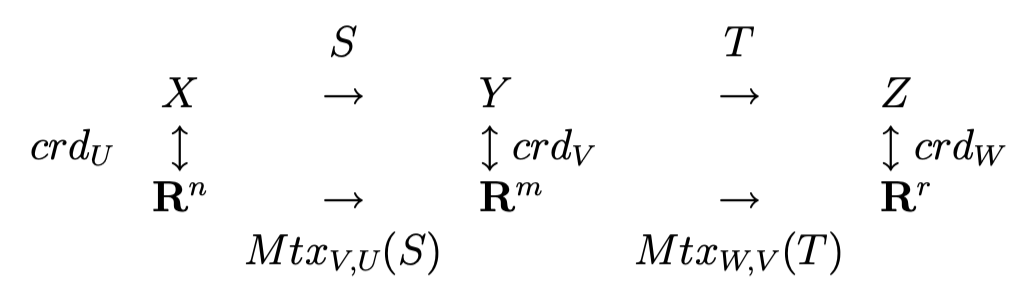
\includegraphics[scale=0.25]{Commutative Diagram.png}
    \caption{Commutative Diagram}
    \label{}
\end{figure}\end{center}
We say the diagram commutes because you get the same answer any way you go around the diagram (in directions allowed by the arrows). The $\textnormal{crd}$ arrows go in both directions because $\textnormal{crd}$ is an isomorphism.


\section{Change of Basis and Similarity}
Let $X$ be a finite-dimensional vector space with basis $V$. If $T \in L(X, X)$ it is customary to use the same basis in the domain and range. In this case, we use $\textnormal{Mtx}_V(T)$ to denotes $\textnormal{Mtx}_{V,V}(T)$.

\subsection{Change of Basis}
\textbf{Question:} If $W$ is another basis for $X$, how are $M t x_V(T)$ and $M t x_W(T)$ related?
$$
\begin{aligned}
\operatorname{Mtx}_{V, W}(i d) \cdot M t x_W(T) \cdot M t x_{W, V}(i d) & =M t x_{V, W}(i d) \cdot M t x_{W, V}(T \circ i d) \\
& =M t x_{V, V}(i d \circ T \circ i d) \\
& =M t x_V(T)
\end{aligned}
$$
and
$$
\begin{aligned}
\operatorname{Mtx}_{V, W}(i d) \cdot M t x_{W, V}(i d) & =M t x_{V, V}(i d)
& =\left(\begin{array}{cccccc}
1 & 0  & \cdots & 0 \\
0 & 1  & \cdots & 0 \\
\vdots & \vdots & \ddots & \vdots \\
0 & 0 & \cdots & 1
\end{array}\right)
\end{aligned}
$$
So this says that
$$
M t x_V(T)=P^{-1} M t x_W(T) P
$$
for the invertible matrix
$$
P=M t x_{W, V}(i d)
$$
that is the change of basis matrix.

On the other hand, if $P$ is any invertible matrix, then $P$ is also a change of basis matrix for appropriate corresponding bases.

\subsection{Similarity}
\begin{definition}[Similar]
    \normalfont
    Square matrices $A$ and $B$ are \textbf{similar} if $$A=P^{-1}BP$$ for some invertible matrix $P$.
\end{definition}


\subsection{Theorem: Similar Matrices $\Leftrightarrow$ Same Linear Transformation for Two Bases}
\begin{theorem}[Similar Matrices $\Leftrightarrow$ Same Linear Transformation for Two Bases]
    Suppose that $X$ is a finite-dimensional vector space.
    \begin{enumerate}
        \item If $T \in L(X, X)$ then any two matrix representations of $T$ are \textbf{similar}. That is, if $U, W$ are any two bases of $X$, then $\textnormal{Mtx}_W(T)$ and $\textnormal{Mtx}_U(T)$ are similar.
        \item Conversely, two similar matrices represent the same linear transformation $T$, relative to suitable bases. That is, given similar matrices $A, B$ with $A = P^{-1}BP$ and any basis $U$, there is a basis $W$ and $T \in L(X, X)$ such that
        \begin{center}
            $B=\textnormal{Mtx}_U(T)$, $A=\textnormal{Mtx}_W(T)$, $P=\textnormal{Mtx}_{U,W}(id)$, $P^{-1}=\textnormal{Mtx}_{W,U}(id)$.
        \end{center}
    \end{enumerate}
\end{theorem}





\section{Square Matrix $A_{n\times n}$: $det(A)$, singular}
\begin{enumerate}
    \item A is singular if $det(A)=0$, else non-singular.
    \item If $det(A)\neq 0$, $A^{-1}$ exists and $A^{-1}=\frac{adj(A)}{det(A)}$
    \item $det(AB)=det(A)det(B)$
\end{enumerate}

\section{Eigenvalues and Eigenvectors}
\begin{definition}[Matrix Form: Eigenvalues, Eigenvectors]
    \normalfont
    A vector $x$ is a $\textbf{eigenvector}$ of a matrix $A$ if $Ax$ is parallel to $x$, that is if $Ax = \lambda x$ for some number $\lambda\in \mathbb{R}$. The number $\lambda$ is called a $\textbf{eigenvalue}$ of $A$.

    i.e. the root of $(A-\lambda I_n)x=0\Leftrightarrow det(A-\lambda I_n)=0$
\end{definition}

\begin{definition}[Linear Transformation: Eigenvalues, Eigenvectors]
    \normalfont
    Let $X$ be a vector space and $T \in L(X, X)$. We say that $\lambda$ is an \textbf{eigenvalue} of $T$ and $v\neq 0$ is an \textbf{eigenvector} corresponding to $\lambda$ if $T (v) = \lambda v$.
\end{definition}


\begin{theorem}[Matrix Form and LT Form are equivalent]
    Let $X$ be a finite-dimensional vector space, and $U$ a basis. Then $\lambda$ is an eigenvalue of $T$ \underline{if and only if} $\lambda$ is an eigenvalue of $\textnormal{Mtx}_U(T)$. $v$ is an eigenvector of $T$ corresponding to $\lambda$ \underline{if and only if} $\textnormal{crd}_U(v)$ is an eigenvector of $\textnormal{Mtx}_U(T)$ corresponding to $\lambda$.
\end{theorem}



\section{Diagonalizable Matrix}
\begin{definition}[Diagonalizable]
    \normalfont
    Suppose $X$ is a finite-dimensional vector space with basis $U$. Given a linear transformation $T\in L(X,X)$, let $$A=\textnormal{Mtx}_U(T)$$
    We say that $A$ can be diagonalized (or is \textbf{diagonalizable}) if there is another basis $W$ for $X$ such that $\textnormal{Mtx}_W(T)$ is diagonal, i.e. $$\textnormal{Mtx}_W(T)=\begin{bmatrix}
        \lambda_1&&&\\
        &\lambda_2&&\\
        &&\ddots&\\
        &&&\lambda_n
    \end{bmatrix}$$
\end{definition}
A $n\times n$ matrix $A$ with $n$ linearly independent eigenvalues $u$ is said to be \textit{diagonalizable}.
\begin{equation}
    \begin{aligned}
        AU&=A\begin{bmatrix}
            |&|&\cdots&|\\
            u_1&u_2&\cdots&u_n\\
            |&|&\cdots&|
        \end{bmatrix}\\
        &=\begin{bmatrix}
            |&|&\cdots&|\\
            \lambda_1u_1&\lambda_2u_2&\cdots&\lambda_nu_n\\
            |&|&\cdots&|
        \end{bmatrix}\\
        &=\begin{bmatrix}
            |&|&\cdots&|\\
            u_1&u_2&\cdots&u_n\\
            |&|&\cdots&|
        \end{bmatrix}\begin{bmatrix}
            \lambda_1&&&\\
            &\lambda_2&&\\
            &&\ddots&\\
            &&&\lambda_n
        \end{bmatrix}\\
        &=UD\\
        \Rightarrow	A&=UDU^{-1}
    \end{aligned}
    \nonumber
\end{equation}

\begin{theorem}
    If an $n\times n$ matrix $A$ has $n$ linearly independent eigenvectors $u_1,...,u_n$ corresponding to eigenvalues $\lambda_1,...,\lambda_n$, then $A = UDU^{-1}$ where $D$ is diagonal with entries $\lambda_1,...,\lambda_n$, and $U$ has columns $u_1,...,u_n$.
\end{theorem}
$A$ is \textbf{similar} to $D$ ($\exists P$ s.t. $A=PDP^{-1}$).

Not \textit{diagonalizable} is also called \textit{defective}.


\begin{theorem}[Diagonalized $\Leftrightarrow$ $\exists$ basis consisiting of eigenvectors]
    Let $X$ be an n-dimensional vector space, $T \in L(X, X)$, $U$ any basis of $X$, and $A = \textnormal{Mtx}_U(T)$. Then the following are equivalent:
    \begin{enumerate}
        \item $A$ can be diagonalized.
        \item There is a basis $W$ for $X$ consisting of eigenvectors of $T$.
        \item There is a basis $V$ for $\mathbb{R}^n$ consisting of eigenvectors of $A$.
    \end{enumerate}
\end{theorem}

\begin{theorem}[Distinct Eigencalues Correspond to Distinct Eigenvectors]
    Let $X$ be a vector space and $T \in L(X, X)$.
    \begin{enumerate}
        \item If $\lambda_1, . . . , \lambda_m$ are distinct eigenvalues of $T$ with corresponding eigenvectors $v_1, . . . , v_m$, then $\{v_1, . . . , v_m\}$ is linearly independent.
        \item If $\dim X = n$ and $T$ has $n$ distinct eigenvalues, then $X$ has a basis consisting of eigenvectors of $T$; consequently, if $U$ is any basis of $X$, then $\textnormal{Mtx}_U(T)$ is diagonalizable.
    \end{enumerate}
\end{theorem}

\begin{corollary}
    An $n\times n$ matrix with $n$ distinct eigenvalues is diagonalizable.
\end{corollary}
(Because the $n$ associated eigenvectors are always linearly independent.)



\section{Orthogonal, Orthonormal, Unitary}
Two vectors $a$ and $b$ are orthogonal, if their dot product is equal to zero (they are perpendicular). $$a\cdot b=0$$

Two vectors $a$ and $b$ are orthonormal, if they are orthogonal \textbf{unit vectors}.

Formally,
\begin{definition}[Orthonormal]
    \normalfont Let $\delta_{ij}=\left\{\begin{matrix}
        1,& \textnormal{ if }i=j\\
        0,& \textnormal{ if }i\neq j
    \end{matrix}\right.$. A basis $V = \{v_1, . . . , v_n\}$ of $\mathbb{R}^n$ is \textbf{orthonormal} if $v_i \cdot v_j = \delta_{ij}$.
\end{definition}


\begin{definition}[Unitary]
    \normalfont
    A real $n \times n$ matrix $A$ is \textbf{unitary} if $A^T=A^{-1}$.
\end{definition}


\begin{theorem}
    A real $n \times n$ matrix $A$ is \textbf{unitary} \underline{if and only if} the columns of $A$ are \textbf{orthonormal}.
\end{theorem}

If $A$ is unitary, let $V$ be the set of columns of $A$ and $W$ be the standard basis of $\mathbf{R}^n$. Since $A$ is unitary, it is invertible, so $V$ is a basis of $\mathbf{R}^n$.
$$
A^{\top}=A^{-1}=\textnormal{Mtx}_{V,M}(id)
$$
where $A=[v_1,...,v_n]$: $A\textnormal{Mtx}_{V,M}(id)=[v_1,...,v_n]\textnormal{Mtx}_{V,M}(id)=[m_1,...,m_n]=\mathbb{I}_{n\times n} \Rightarrow \textnormal{Mtx}_{V,M}(id)=A^{-1}$.

Since $V$ is orthonormal, the transformation between bases $W$ and $V$ preserves all geometry, including lengths and angles.





\section{Eigen Decomposition of Symmetric Matrices Results}
Let A be a symmetric $n\times n$ matrix, i.e. $A^T=A$
\begin{proposition}
All eigenvalues of $A$ are real.
\end{proposition}
\begin{proposition}
Eigenvectors corresponding to distinct eigenvalues are orthogonal.
\end{proposition}
\begin{proof}
\quad

Let $\lambda_1$, $\lambda_2$ be eigenvalues s.t. $\lambda_1\neq\lambda_2$.
$$Au_1=\lambda_1 u_1;\ Au_2=\lambda_2 u_2$$
\begin{equation}
    \begin{aligned}
        \lambda_1 u_1^Tu_2&=(Au_1)^Tu_2=u^T_1A^Tu_2\\
        &=u^T_1Au_2=u^T_1(Au_2)=\lambda_2 u^T_1u_2\\
        &\Rightarrow	u_1^Tu_2=0\text{ Since }\lambda_1\neq\lambda_2
    \end{aligned}
    \nonumber
\end{equation}
\end{proof}

\begin{proposition}
If $\lambda$ is an eigenvalue with multiplicity $k$, we can find $k$ orthogonal eigenvectors for $\lambda$.
\end{proposition}
Multiplicity: the number of times an element is repeated in a multiset.

\section{Diagonalization of Real Symmetric Matrices}
\begin{theorem}[Diagonalization of Real Symmetric Matrices]
    Let $T \in L\left(\mathbf{R}^n, \mathbf{R}^n\right)$ and $W$ be the standard basis of $\mathbf{R}^n$. Suppose that $M t x_W(T)$ is symmetric. Then the eigenvectors of $T$ are all real, and there is an orthonormal basis $V=\left\{v_1, \ldots, v_n\right\}$ of $\mathbf{R}^n$ consisting of eigenvectors of $T$, so that $M t x_W(T)$ is diagonalizable:
    $$
    M t x_W(T)=M t x_{W, V}(i d) \cdot M t x_V(T) \cdot M t x_{V, W}(i d)
    $$
    where $M t x_V (T)$ is diagonal and the change of basis matrices $M t x_{V, W}(i d)$ and $M t x_{W, V}(i d)$ are unitary.
\end{theorem}
A real symmetric matrix $A_{n\times n}$ can be written as
\begin{equation}
    \begin{aligned}
        A&=\sum_{i=1}^n\lambda_i u_iu_i^T=U\Omega U^T
    \end{aligned}
    \nonumber
\end{equation}
$u_i$ are orthonormal eigenvectors. $\lambda_i$ are eigenvalues.

Where $U=[u_1,u_2,...,u_n]$, $\Omega=diag(\lambda_1,...,\lambda_n)$

Since $u_i$ are orthonormal eigenvectors, $U^TU=I \Rightarrow U^T=U^{-1}$. $U$ is an orthogonal matrix.

\subsection{Proposition: $\lambda_{\min}\|x\|^2\leq x^TAx\leq \lambda_{\max}\|x\|^2$}
\begin{proposition}
For any $x\in \mathbb{R}^n$, $$\lambda_{\min}\|x\|^2\leq x^TAx\leq \lambda_{\max}\|x\|^2$$
\end{proposition}
\begin{proof}
    Since $u_i$ are orthonormal and linearly independent. $x=\sum_{i=1}^n\alpha_i u_i$ for some $\alpha_i\in \mathbb{R},i=1,...,n$
    \begin{equation}
        \begin{aligned}
            x^TAx&=(\sum_{i=1}^n\alpha_i u_i)^TA(\sum_{j=1}^n\alpha_j u_j)\\
            &=\sum_{i=1}^n\sum_{j=1}^n\alpha_i \alpha_ju_i^TAu_j\\
            &=\sum_{i=1}^n\sum_{j=1}^n\alpha_i \alpha_ju_i^T(Au_j)\\
            &=\sum_{i=1}^n\alpha_i^2\lambda_i\\
            \Rightarrow	\lambda_{\min}\|x\|^2&\leq x^TAx\leq \lambda_{\max}\|x\|^2
        \end{aligned}
        \nonumber
    \end{equation}
    The first equation holds if $x$ is the eigenvector for $\lambda_{\min}$. The second equation holds if $x$ is the eigenvector for $\lambda_{\max}$.
\end{proof}

\subsection{Proposition: $\lambda^2$ is the eigenvalue of $A^2$ and $A^TA$}
\begin{proposition}
If $\lambda$ is an eigenvalue of $A$, then $\lambda^2$ is the eigenvalue of $A^2$ and $ A^TA$, the corresponding eigenvector doesn't change.
\end{proposition}
\begin{proof}
\begin{equation}
    \begin{aligned}
        Ax_1&=\lambda x_1\\
        A^2x_1=A(Ax_1)=\lambda Ax_1&=\lambda^2 x_1\\
        A^TAx_1=A^T(Ax_1)=\lambda A^Tx_1&=\lambda^2x_1
    \end{aligned}
    \nonumber
\end{equation}
\end{proof}

\section{Trace}
$A_{n\times n}$, $Tr(A)=\sum_{i=1}^nA_{kk}$
$$det(A)=\prod_{i=1}^n\lambda_i,\ Tr(A)=\sum_{i=1}^n\lambda_i$$
\begin{proposition}[Invariance Property]
$A_{m\times n}$, $B_{n\times k}$, $C_{k\times m}$, $Tr(ABC)=Tr(CAB)=Tr(BCA)$.
\end{proposition}






\section{Jacobian matrix}
Suppose $\mathbf{f}: \mathbf{R}^{n} \rightarrow \mathbf{R}^{m}$ is a function such that each of its first-order partial derivatives exist on $\mathbf{R}^{n}.$ This function takes a point $\mathbf{x} \in \mathbf{R}^{n}$ as input and produces the vector $\mathbf{f}(\mathbf{x}) \in \mathbf{R}^{m}$ as output. Then the Jacobian matrix of $\mathbf{f}$ is defined to be an $m \times n$ matrix, denoted by $\mathbf{J}$, whose $(i, j)$ th entry is $\mathbf{J}_{i j}=\frac{\partial f_{i}}{\partial x_{j}}$, or explicitly

$
\mathbf{J}=\left[\begin{array}{ccc}
\frac{\partial \mathbf{f}}{\partial x_{1}} & \cdots & \frac{\partial \mathbf{f}}{\partial x_{n}}
\end{array}\right]=\left[\begin{array}{c}
\nabla^{\mathrm{T}} f_{1} \\
\vdots \\
\nabla^{\mathrm{T}} f_{m}
\end{array}\right]=\left[\begin{array}{ccc}
\frac{\partial f_{1}}{\partial x_{1}} & \cdots & \frac{\partial f_{1}}{\partial x_{n}} \\
\vdots & \ddots & \vdots \\
\frac{\partial f_{m}}{\partial x_{1}} & \cdots & \frac{\partial f_{m}}{\partial x_{n}}
\end{array}\right]
$

where $\nabla^{\mathrm{T}} f_{i}$ is the transpose (row vector) of the gradient of the $i$ component.

\section{Hessian matrix}
Suppose $f: \mathbb{R}^{n} \rightarrow \mathbb{R}$ is a function taking as input a vector $\mathbf{x} \in \mathbb{R}^{n}$ and outputting a scalar $f(\mathbf{x}) \in \mathbb{R}$. If all second partial derivatives of $f$ exist and are continuous over the domain of the function, then the Hessian matrix $\mathbf{H}$ of $f$ is a square $n \times n$ matrix, usually defined and arranged as follows:

$
\mathbf{H}_{f}=\left[\begin{array}{cccc}
\frac{\partial^{2} f}{\partial x_{1}^{2}} & \frac{\partial^{2} f}{\partial x_{1} \partial x_{2}} & \cdots & \frac{\partial^{2} f}{\partial x_{1} \partial x_{n}} \\
\frac{\partial^{2} f}{\partial x_{2} \partial x_{1}} & \frac{\partial^{2} f}{\partial x_{2}^{2}} & \cdots & \frac{\partial^{2} f}{\partial x_{2} \partial x_{n}} \\
\vdots & \vdots & \ddots & \vdots \\
\frac{\partial^{2} f}{\partial x_{n} \partial x_{1}} & \frac{\partial^{2} f}{\partial x_{n} \partial x_{2}} & \cdots & \frac{\partial^{2} f}{\partial x_{n}^{2}}
\end{array}\right],
$

or, by stating an equation for the coefficients using indices $i$ and $j$,

$
\left(\mathbf{H}_{f}\right)_{i, j}=\frac{\partial^{2} f}{\partial x_{i} \partial x_{j}}.
$

The Hessian matrix is a symmetric matrix, since the hypothesis of continuity of the second derivatives implies that the order of differentiation does not matter (Schwarz's theorem).

The determinant of the Hessian matrix is called the Hessian determinant.

\section{Positive Definite Matrices}
\subsection{Definition}
We say that a symmetric $n \times n$ matrix $A$ is:

(1). $\textbf{ positive semidefinite (PSD)}$ (written $A \succeq 0$) if $x^TAx \geq 0$ for all $x$.

(2). $\textbf{ positive definite (PD)}$ (written $A \succ 0$) if $x^TAx > 0$ for all $x\neq 0$.

(3). $\textbf{ negative semidefinite (NSD)}$ (written $A \preceq 0$) if $x^TAx \leq 0$ for all $x$.

(4). $\textbf{ negative definite (ND)}$ (written $A \prec 0$) if $x^TAx < 0$ for all $x\neq 0$.

(5). $\textbf{ indefinite}$ (not written in any particular way) if none of the above apply.

$x^TAx$ is a function of $x$ called the quadratic form associated to $A$.

$A$ is ND(NSD) $\Leftrightarrow$ $-A$ is PD(PSD)

$\textbf{Note:}$ $A^TA$ is $\textbf{ positive semidefinite}$, since $x^TA^TAx=\|Ax\|^2\geq 0$.

$\textbf{Note:}$ We can extend definition to non-symmetric $n\times n$
\begin{equation}
    \begin{aligned}
        x^TAx=x^TA^Tx \Rightarrow x^TAx=x^T(\frac{A+A^T}{2})x
    \end{aligned}
    \nonumber
\end{equation}

\subsection{Condition number (for PD matrix)}
Condition number (for PD matrix):$$\kappa (A)=\frac{\lambda_{max}}{\lambda_{min}}>0$$











\subsection{Diagonal matrix situation}
$$D=\begin{bmatrix}
    d_1&0&... &0\\0&d_2&...&0\\...&...&...&...\\0&0&...&d_n
\end{bmatrix}$$
\begin{lemma}
    If $d_1,...d_n$ are all nonnegative, then $D\succeq 0$;

    If $d_1,...d_n$ are all positive, then $D\succ 0$;
    
    If $d_1,...d_n$ are all nonpositive, then $D\preceq 0$;
    
    If $d_1,...d_n$ are all negative, then $D\prec 0$;
\end{lemma}

\subsection{Using eigenvalues}
If $A$ is an $n \times n$ symmetric matrix, then it can be factored as
    $$A=Q^T\Lambda Q=Q^T
    \begin{bmatrix}
        \lambda_1&0&... &0\\
        0&\lambda_2&...&0\\
       ...&...&...&...\\
        0&0&...&\lambda_n
    \end{bmatrix}Q$$

where $\lambda_1,..., \lambda_n$ are the eigenvalues of $A$ and the columns of $Q$ are the corresponding eigenvectors.

    We can get $x^TAx=x^TQ^T\Lambda Qx=(Qx)^T\Lambda(Qx)$
    
    If we substitute $y=Qx$:
    
    $x^TAx=y^T\Lambda y=\lambda_1y_1^2+\lambda_2y_2^2+...+\lambda_ny_n^2$

\begin{theorem}
    \quad

    If $\lambda_1,...\lambda_n$ are all non-negative, then symmetric matrix $A\succeq 0$;
    
    If $\lambda_1,...\lambda_n$ are all positive, then $A\succ 0$;
    
    If $\lambda_1,...\lambda_n$ are all non-positive, then $A\preceq 0$;
    
    If $\lambda_1,...\lambda_n$ are all negative, then $A\prec 0$;
    
    if it has both positive and negative eigenvalues, then $A$ is indefinite
\end{theorem}

\subsection{Sylvester’s Criterion}

Consider a $n\times n$ matrix $A$: $$A=\begin{bmatrix}
    a_{11}&a_{12}&... &a_{1n}\\a_{21}&a_{22}&...&a_{2n}\\...&...&...&...\\a_{n1}&a_{n2}&...&a_{nn}
\end{bmatrix}$$

Denote its $k\times k$ submatrix $A^{(k)}$:
$$A^{(k)}=\begin{bmatrix}
    a_{11}&a_{12}&... &a_{1k}\\a_{21}&a_{22}&...&a_{2k}\\...&...&...&...\\a_{k1}&a_{k2}&...&a_{kk}
\end{bmatrix}$$

Let $\Delta_k=det(A^{(k)})$

$$det(A-xI)=(\lambda_1-x)(\lambda_2-x)...(\lambda_n-x)$$
by setting $x = 0$ we get $det(A) = \lambda_1\lambda_2...\lambda_n$.

When $A\succ 0$, all the eigenvalues are positive, so $det(A) > 0$ as well.

$A\succ 0\Rightarrow \vec{x}^TA\vec{x}>0$ for all $\vec{x}\neq \vec{0}$. Consider $\vec{x}\in \mathbb{R}^n$ with $x_{k+1}=\cdots=x_n=0$. $\vec{x}=[x_1,x_2,...,x_k,0,...0]^T$. Then,
$$\vec{x}^TA\vec{x}=[x_1,x_2,...,x_k,0,...0]\begin{bmatrix}
    a_{11}&a_{12}&... &a_{1n}\\a_{21}&a_{22}&...&a_{2n}\\...&...&...&...\\a_{n1}&a_{n2}&...&a_{nn}
\end{bmatrix}\begin{bmatrix}
    x_1\\
    \vdots\\
    x_k\\
    0\\
    \vdots\\
    0
\end{bmatrix}=\vec{x}^TA^{(k)}\vec{x}$$
Then we know $A\succ 0 \Rightarrow A^{(k)}\succ 0$

We expect $A^{(k)}\succ 0\Rightarrow \Delta_k>0$ for all $k$.

\begin{theorem}[Sylvester’s criterion]Let $A$ be $n\times n$ symmetric matrix
    \begin{enumerate}
        \item $A\succ 0$ iff $\Delta_i>0\ \forall i=1,...,n$
        \item $A\prec 0$ iff $(-1)^i\Delta_i>0\ \forall i=1,...,n$
        \item $A$ is indefinite if the first $\Delta_k$that breaks each pattern respectively is the wrong sign (rather than 0).
    \end{enumerate}
\end{theorem}
\begin{proposition}
    \quad

\begin{enumerate}
    \item Symmetric matrix $A$ is PD

    $\Leftrightarrow$ All eigenvalues of $A$ are $>0$
    
    $\Leftrightarrow$ $\Delta_i>0\ \forall i=1,...,n$
    \item Symmetric matrix $A$ is PSD

    $\Leftrightarrow$ All eigenvalues of $A$ are $\geq 0$
    
    $\Leftrightarrow$ $\Delta_i\geq 0\ \forall i=1,...,n$
    \item For ND and NSD, test $-A$ instead of $A$
\end{enumerate}
\end{proposition}

\section{Matrix Norm (Induced Norm) and Spectral Radius}
$\|A\|=\max _{\|x\|=1}\|A x\|$. i.e., find the column with the highest sum of absolute values.

Spectral Radius: for $n\times n$ matrix $A$, $$S(A)=\max_{i=1,...,n}|\lambda_i|$$

\begin{proposition}
$S(A)\leq \|A\|$
\end{proposition}
\begin{proof}
\begin{equation}
    \begin{aligned}
        \|A\|=\max _{\|x\|=1}\|A x\|\geq \|Au\|=|\lambda|\|u\|=|\lambda|
    \end{aligned}
    \nonumber
\end{equation}
\end{proof}

\begin{proposition}
    For symmetric $A_{n\times n}$, $S(A)= \|A\|$
\end{proposition}
\begin{proof}
\quad

$\forall x\in \mathbb{R}^n$, decompose it by $u_i$.
Since $u_i$ are orthonormal and linearly independent. $x=\sum_{i=1}^n\alpha_i u_i$ for some $\alpha_i\in \mathbb{R},i=1,...,n$. $\|x\|^2=\sum_{i=1}^n|\alpha_i|^2$

\begin{equation}
    \begin{aligned}
        \|Ax\|^2&=\|\sum_{i=1}^n\alpha_i A u_i\|^2=\|\sum_{i=1}^n\alpha_i \lambda_i u_i\|^2=\sum_{i=1}^n|\alpha_i|^2|\lambda_i|^2\\
        &\leq \sum_{i=1}^n|\alpha_i|^2S(A)^2=S(A)^2 \Rightarrow	\|A\|\leq S(A)
    \end{aligned}
    \nonumber
\end{equation}

Since we proved $S(A)\leq \|A\|$ before, $S(A)=\|A\|$.
\end{proof}


\chapter{Linear Maps between Normed Spaces}
\begin{definition}[Bounded Linear Transformation]
    \normalfont
    Suppose $X, Y$ are normed vector spaces and $T \in L(X, Y)$. We say $T$ is \textbf{bounded} if $$\exists \beta\in \mathbb{R} \textnormal{ s.t. }\|T(x)\|_Y\leq\beta\|x\|_X, \forall x\in X$$
    Note this implies that $T$ is Lipschitz with constant $\beta$.
\end{definition}

\begin{theorem}
    Let $X, Y$ be normed vector spaces and $T \in L(X, Y)$. Then
    \begin{equation}
        \begin{aligned}
            &\textnormal{$T$ is continuous at some point $x_0 \in X$}\\
            \Leftrightarrow&\textnormal{$T$ is continuous at every $x \in X$}\\
            \Leftrightarrow&\textnormal{$T$ is uniformly continuous on $X$}\\
            \Leftrightarrow&\textnormal{$T$ is Lipschitz}\\
            \Leftrightarrow&\textnormal{$T$ is bounded}
        \end{aligned}
        \nonumber
    \end{equation}
\end{theorem}

\begin{note}
    Every linear map on a finite-dimensional normed vector space is bounded (and thus continuous, uniformly continuous, and Lipschitz continuous).
\end{note}
\begin{theorem}[LP in finite-dimensional normed vector space is bounded]
    Let $X, Y$ be normed vector spaces with dim $X = n$. Every $T \in L(X, Y)$ is bounded (and thus continuous, uniformly continuous, and Lipschitz continuous).
\end{theorem}

\begin{definition}[Topological Isomorphism]
    \normalfont
    A \textbf{topological isomorphism} between normed vector spaces $X$ and $Y$ is a linear transformation $T \in L(X, Y)$ that is \underline{invertible (one-to-one, onto)}, \underline{continuous}, and has a \underline{continuous inverse}.

    Two normed vector spaces $X$ and $Y$ are \textbf{topologically isomorphic} if there is a topological isomorphism $T : X \rightarrow Y$.
\end{definition}

Suppose $X$ and $Y$ are normed vector spaces. We define
\begin{equation}
    \begin{aligned}
        B(X,Y)= \{T \in L(X, Y) : T\textnormal{ is bounded}\}
    \end{aligned}
    \nonumber
\end{equation}
and
\begin{equation}
    \begin{aligned}
        \|T\|_{B(X,Y)}=\sup\left\{\frac{\|T(x)\|_Y}{\|x\|_X},x\in X, x\neq 0\right\}
    \end{aligned}
    \nonumber
\end{equation}








\chapter{Euclidean geometry basics}
\section{Norm}
\subsection{Vector's Norm}
Vector $x \in \mathbb{R}^{n}$-n-dim Euclidean space
$$
x=\left(x_{1}, \ldots, x_{n}\right) \equiv\left[\begin{array}{llll}
x_{1} & x_{2} & \ldots & x_{n}
\end{array}\right]^{\top}=\left[\begin{array}{c}
x_{1} \\
x_{2} \\
\vdots \\
x_{n}
\end{array}\right]
$$

Norm of $x$, $\|x\|$ satisfies properties:

$$
\begin{aligned}
&\text { (a) }\|x\| \geqslant 0 \\
&\text { (b) }\|x\|=0 \Leftrightarrow x=0 \\
&\text { (c) }\|c x\|=|c|\|x\| \text {, for } c \in \mathbb{R} \\
&\text { (d) }\|x+y\| \leqslant\|x\|+\|y\| \longleftarrow \text { Triangle Ineq. }
\end{aligned}
$$

Enclidean Norm (default $\rho=2$): $\|x\|=\sqrt{x^{\top} x}=\sqrt{\sum_{i=1}^{n} x_{i}{ }^{2}}$

Other norms:

1. $l_{1}$-norm : $\|x\|_{1}=\sum_{i=1}^{n}\left|x_{i}\right|$

2. $l_{\rho}$-norm : $\|x\|_{\rho}=\sqrt[\rho]{\sum_{i=1}^{n}\left|x_{i}\right|^\rho}$

3. Supremum norm or $l_{\infty}$-norm : $\|x\|_{\infty}=\max _{i}\left|x_{i}\right|$

\subsection{Matrix's Norm}
$A\in \mathbb{R}^{n\times m}$ is a matrix

$\|A x\| \leqslant\|A\|\|x\|,\|A B\| \leqslant\|A\|\|B\|$

Default is $\rho=1$: $\|A\|=\max _{\|x\|=1}\|A x\|$.

$\|A\|_{F}=\sqrt{\sum_{i, j} a_{i j}^{2}} \quad$ (Frobenius norm);  Frobenius norm property: $\|A\|_F^2=<A,A>=trace(A^TA)$

$\|A\|_{1}=\max _{j} \sum_{i=1}^{n}\left|A_{i j}\right|$ i.e., find the column with the highest sum of absolute values.

$\|A\|_{\infty}=\max _{j} \sum_{j=1}^{n}\left|A_{i j}\right|$ i.e., find the row with the highest sum of absolute values.

${\displaystyle \|A\|_{2}={\sqrt {\lambda _{\max }\left(A^{T}A\right)}}=\sigma _{\max }(A).}$
$\|A\|_{2}=\max _{k} \sigma_{k}. \sigma_{k}$ is the \underline{singular value} (square root of $A^TA$) of $A$ (spectral norm, Euclidean norm)

$\|A\|=\max \left(\frac{\|A x\|}{\|x\|}\right) \Rightarrow\|A\| \geqslant \frac{\|A x\|}{\|x\|}$, $\|Ax\| \leqslant\|A\|\|x\|$

\subsection{Difference between Spectral Radius and Spectral Norm}
Spectral Radius: $S(A)=\max_{i=1,...,n}|\lambda_i|$; Spectral Norm: $\|A\|_{2}=\max _{k} \sigma_{k}$

For real symmetric matrices, $\|A\|_2=S(A)$.

For general matrices, $\|A\|_2\geq S(A)$.

\section{ Euclidean distance, inner product}
\textbf{Euclidean distance} on $\mathbb{R}^n$:
\begin{equation}
    \begin{aligned}
        |x-y|=\sqrt{(x_1-y_1)^2+...+(x_n-y_n)^2}
    \end{aligned}
    \nonumber
\end{equation}
\textbf{Euclidean inner product}:
\begin{equation}
    \begin{aligned}
        x\cdot y=x_1y_1+\cdots +x_ny_n=x^Ty
    \end{aligned}
    \nonumber
\end{equation}
Also written as $<x,y>$

Useful fact: $$<x,y>=\cos(\theta)\|x\|_2\|y\|_2$$
$\theta$ is the angle between $x$ and $y$.

Two important results for Euchidean norm:

1) Pythagorean Theorem: If $x^{\top} y=0$,
\[ \|x+y\|^{2}=\|x\|^{2}+\|y\|^{2} \]

2) Cauchy - Schwarz Inequality:

$$
\begin{aligned}
&<x,y>=\left|x^{\top} y\right| \leqslant\|x\|_2\|y\|_2 \\
&"=" \text { iff } x=\alpha y \text { for some } \alpha \in \mathbb{R}
\end{aligned}
$$

\section{General Inner Products}
\subsection{ Inner Product}
\begin{definition}\end{definition}
An \textbf{inner product $*$} is a function that maps two vectors $\vec{x},\vec{y}\in \mathbb{R}^n$ to a single value $\vec{x}*\vec{y}\in \mathbb{R}$, satisfying the following axioms:
\begin{enumerate}
    \item \textbf{Bilinear} (linearity in both arguments): for all $\vec{x},\vec{y},\vec{z}\in \mathbb{R}^n$ and $a,b\in \mathbb{R}$, we have
    \begin{equation}
        \begin{aligned}
            (a \vec{x}+ b\vec{y})*\vec{z}&=a(\vec{x}*\vec{z})+b(\vec{xy}*\vec{z})\\
            \vec{x}*(a \vec{y}+b \vec{z})&=a(\vec{x}* \vec{y})+ b(\vec{x}* \vec{z})
        \end{aligned}
        \nonumber
    \end{equation}
    \item \textbf{Symmetric} i.e. for all $\vec{x},\vec{y}\in \mathbb{R}^n$, $$\vec{x}* \vec{y}=\vec{y}* \vec{x}$$
    \item \textbf{Positivity} i.e. for all $\vec{x}\in \mathbb{R}^n$, $$\vec{x}* \vec{x}\geq 0$$ with equality if and only if $\vec{x}=\vec{0}$
\end{enumerate}

\begin{definition}
    Every inner product $*$ defines a corresponding norm $\|\cdot\|_*$ as $\|\vec{x}\|_*=\sqrt{\vec{x}*\vec{x}}$
\end{definition}

\subsection{Theorem: $*$ is inner product iff $\vec{x}*\vec{y}=\vec{x}^T H \vec{y}$ for some symmetric $H$}
\begin{theorem}
    An operation $*: \mathbb{R}^n\times \mathbb{R}^n \rightarrow  \mathbb{R}$ is an inner product if and only if it can be written as $\vec{x}*\vec{y}=\vec{x}^T H \vec{y}$ for some symmetric positive definite $n\times n$ matrix $H$.
\end{theorem}
\begin{proof}
Define $H:=[H_{ij}]=[\vec{e}_i*\vec{e}_j]$
\begin{enumerate}
    \item Bilinear:
    \begin{equation}
        \begin{aligned}
            \vec{x}*\vec{y}&=\left(\sum_{i=1}^nx_i \vec{e}_i\right)*\left(\sum_{j=1}^ny_j \vec{e}_j\right)\\
            &=\sum_{i=1}^nx_i\left(\vec{e}_i*\sum_{j=1}^ny_j \vec{e}_j\right)\quad \text{(by linearity)}\\
            &=\sum_{i=1}^nx_i\left(\sum_{j=1}^ny_j(\vec{e}_i* \vec{e}_j)\right)\quad \text{(by linearity)}\\
            &=\sum_{i=1}^n\sum_{j=1}^nx_i\left(\vec{e}_i* \vec{e}_j\right)y_j\\
            &=\sum_{i=1}^n\sum_{j=1}^nx_iH_{ij}y_j
            =\vec{x}^T H \vec{y}
        \end{aligned}
        \nonumber
    \end{equation}
    \item Symmetric $\Leftrightarrow$ $H=H^T$:
    \begin{equation}
        \begin{aligned}
            \vec{x}* \vec{y}=\vec{x}^TH \vec{y}=\left(\vec{x}^T H \vec{y}\right)^T= \vec{y}^T H^T \vec{x}= \vec{y}^T H \vec{x}=\vec{y}* \vec{x}
        \end{aligned}
        \nonumber
    \end{equation}
    \item Positivity $\Leftrightarrow$ $H\succ 0$: $\vec{x}^T H \vec{x}\geq 0$ with equality only if $\vec{x}=0$
\end{enumerate}
\end{proof}
As we know that a symmetric matrix $H$ is positive definite if and only if we can write $H=B^TB$ for some invertible matrix $B$.
\begin{equation}
    \begin{aligned}
        \vec{x}*\vec{y}=\vec{x}^T H \vec{y}=\vec{x}^T B^T B \vec{y}=(B \vec{x})^T B \vec{y}=(B \vec{x})\cdot (B \vec{y})
    \end{aligned}
    \nonumber
\end{equation}

\begin{definition}
    Given a positive definite matrix $H$, let the associated inner product be $\vec{x}\cdot_H \vec{y}= \vec{x}^T H \vec{y}$ and the associated norm be $\|\vec{x}\|_H=\sqrt{\vec{x}^T H \vec{x}}$
\end{definition}
















\section{Isometry}
An \textbf{isometry} of $\mathbb{R}^n$ is a bijection $\varPhi :\mathbb{R}^n \rightarrow \mathbb{R}^n$ that preserves distance, which means,
\begin{equation}
    \begin{aligned}
        |\varPhi(x)-\varPhi(y)|=|x-y|,\ \forall x,y\in \mathbb{R}^n
    \end{aligned}
    \nonumber
\end{equation}
We use $\textnormal{Isom}(\mathbb{R}^n)$ denotes the set of all isometries of $\mathbb{R}^n$,
\begin{equation}
    \begin{aligned}
        \textnormal{Isom}(\mathbb{R}^n)=\{\varPhi:\mathbb{R}^n \rightarrow \mathbb{R}^n | |\varPhi(x)-\varPhi(y)|=|x-y|,\ \forall x,y\in \mathbb{R}^n\}
    \end{aligned}
    \nonumber
\end{equation}


\begin{proposition}
$\varPhi, \varPsi \in \textnormal{Isom}(\mathbb{R}^n)$, then $\varPhi\circ\varPsi, \varPhi^{-1}\in \textnormal{Isom}(\mathbb{R}^n)$
\end{proposition}
\begin{proof}
\quad\\
Since $\varPhi,\varPsi$ are bijections, so is $\varPhi\circ\varPsi$. Moreover,\\
\begin{equation}
    \begin{aligned}
        &|\varPhi\circ\varPsi(x)-\varPhi\circ\varPsi(y)|=|\varPhi(\varPsi(x))-\varPhi(\varPsi(y))|=|\varPsi(x)-\varPsi(y)|=|x-y|\\
    \end{aligned}
    \nonumber
\end{equation}
Since $id\in \textnormal{Isom} (\mathbb{R}^n)$,
\begin{equation}
    \begin{aligned}
        |x-y|=|id(x)-id(y)|=|\varPhi\circ\varPhi^{-1}(x)-\varPhi\circ\varPhi^{-1}(y)|=|\varPhi^{-1}(x)-\varPhi^{-1}(y)|
    \end{aligned}
    \nonumber
\end{equation}
\end{proof}

\section{ Linear isometries i.e. orthogonal group}
There is a matrix $A\in GL(n,\mathbb{R})$ i.e. a \textit{invertible linear transofrmations} $T_A: \mathbb{R}^n \rightarrow \mathbb{R}^n$ is given by $T_A(v)=Av$.
\begin{equation}
    \begin{aligned}
        T_A(v)\cdot T_A(w)=(Av)\cdot(Aw)=(Av)^t(Aw)=v^tA^tAw
    \end{aligned}
    \nonumber
\end{equation}
\begin{equation}
    \begin{aligned}
        A^tA=I\Leftrightarrow T_A(v)\cdot T_A(w)=v\cdot \Leftrightarrow T_A\in \textnormal{Isom}(\mathbb{R}^n)
    \end{aligned}
    \nonumber
\end{equation}
We define the all isometries in \textit{invertible linear transofrmations} $\mathbb{R}^n \rightarrow \mathbb{R}^n$ as \textbf{orthogonal group}
\begin{equation}
    \begin{aligned}
        O(n)=\{A\in GL(n,\mathbb{R})|A^tA=I \}\subset GL(n,\mathbb{R})
    \end{aligned}
    \nonumber
\end{equation}

\section{Special orthogonal group}
$O(n)$ are the matrices representing linear isometries of $\mathbb{R}^n$.
$1=det(I)=det(A^tA)=det(A^t)det(A)=det(A)^2 \Rightarrow	det(A)=1$ or $det(A)=-1$. We use \textbf{special orthogonal group} represents $A$ with $det(A)=1$,
\begin{equation}
    \begin{aligned}
        SO(n)=\{A\in O(n) | det(A)=1\}
    \end{aligned}
    \nonumber
\end{equation}

\section{Translation}
Define a \textit{translation} by $v\in \mathbb{R}^n$,
\begin{equation}
    \begin{aligned}
        \tau_v:\mathbb{R}^n \rightarrow \mathbb{R}^n,\ \tau_v(x)=x+v
    \end{aligned}
    \nonumber
\end{equation}
\begin{note}[Exercise 2.5.3]
$\forall v\in \mathbb{R}^n, \tau_v$ is an isometry.
\end{note}
\begin{proof}
$|\tau_v(x)-\tau_v(y)|=|(x+v)-(y+v)|=|x-y|$
\end{proof}

\section{All isometries can be represented by a composition of \textit{a translation} and \textit{an orthogonal transformation}}
Since \textit{the composition of isometries is an isometry,} $\forall A\in O(n)$ and $v\in \mathbb{R}^n$, the composition
\begin{equation}
    \begin{aligned}
        \Phi_{A,v}(x)=\tau_v(T_A(x))=Ax+v
    \end{aligned}
    \nonumber
\end{equation}
is an isometry. \textbf{which could account for all isometries}.
\begin{theorem}
$\textnormal{Isom}(\mathbb{R}^n)=\{\Phi_{A,v}|A\in O(n), v\in \mathbb{R}^n \}$
\end{theorem}

\chapter{Algebra Computation}
\section{Hessian Matrix}
\begin{definition}
    The Hessian of $f$ at point $x$ is an $n\times n$ symmetric matrix denoted by $\nabla^2 f(x)$ with $[\nabla^2 f(x)]_{ij}=\frac{\partial^2 f(x)}{\partial x_i\partial x_j}$
\end{definition}

\section{Taylor's Expansion}
\begin{definition}[Taylor's Expansion of Vector]
    $$f(y)-f(x)=\nabla f(x)^T(y-x)+\frac{1}{2}(x-y)^T \nabla^2 f(x)(x-y)+o(\|x-y\|^2)$$
\end{definition}
\section{ Random Vectors and Random Matrices}
\subsection{Mean}
\begin{definition}[Mean of a random vector]
    The mean of a $d-$dimensional random vector $\vec{x}$ is
    $$\mathbb{E}(\vec{x})=\begin{pmatrix}
        \mathbb{E}(x_1)\\
        \mathbb{E}(x_2)\\
        \cdots\\
        \mathbb{E}(x_d)
    \end{pmatrix}$$
\end{definition}

\begin{definition}[Mean of a random matrix]
    The mean of a $d_1\times d_2$ matrix with random entries $\vec{X}$ is
    $$\mathbb{E}(\vec{X})=\begin{pmatrix}
        \mathbb{E}(\vec{X}[1,1])&\mathbb{E}(\vec{X}[1,2])&\cdots &\mathbb{E}(\vec{X}[1,d_2])\\
        \mathbb{E}(\vec{X}[2,1])&\mathbb{E}(\vec{X}[2,2])&\cdots &\mathbb{E}(\vec{X}[2,d_2])\\
        \cdots&\cdots&\cdots&\cdots\\
        \mathbb{E}(\vec{X}[d_1,1])&\mathbb{E}(\vec{X}[d_1,2])&\cdots &\mathbb{E}(\vec{X}[d_1,d_2])\\
    \end{pmatrix}$$
\end{definition}

\begin{lemma}[Linearity of expectation for random vectors and matrices]
    Let $\vec{x}$ be a $d-$dimensional random vector and $b\in \mathbb{R}^{m}$ and $A\in \mathbb{R}^{m\times d}$, then
    \begin{equation}
        \begin{aligned}
            \mathbb{E}(A \vec{x}+b)=A \mathbb{E}(\vec{x})+b
        \end{aligned}
        \nonumber
    \end{equation}
    Similarly let, $\vec{X}$ be a $d_1 \times d_2$ random matrix and $B\in \mathbb{R}^{m\times d_2}$ and $A\in \mathbb{R}^{m\times d_1}$, then
    \begin{equation}
        \begin{aligned}
            \mathbb{E}(A \vec{X}+B)=A \mathbb{E}(\vec{X})+B
        \end{aligned}
        \nonumber
    \end{equation}
\end{lemma}

\begin{definition}[Sample mean of multivariate data]
    Let $X := \{x_1, x_2,..., x_n\}$ denote a set of $d-$dimensional vectors of real-valued data. The sample mean is the entry-wise average
    \begin{equation}
        \begin{aligned}
            \mu_X:=\frac{\sum_{i=1}^n x_i}{n}
        \end{aligned}
        \nonumber
    \end{equation}
\end{definition}

\subsection{Variance, Covariance}
\begin{definition}[Covariance matrix of a vector]
    The covariance matrix of a $d-$dimensional random vector $\vec{x}$ is the $d\times d$ matrix
    \begin{equation}
        \begin{aligned}
            \Sigma_{\vec{x}}=\mathbb{E}[(\vec{x}-\mathbb{E}(\vec{x}))^T(\vec{x}-\mathbb{E}(\vec{x}))]=\begin{bmatrix}
                \textnormal{Var}(\vec{x}[1])&\cdots	&\textnormal{Cov}(\vec{x}[1],\vec{x}[d])\\
                \cdots&\cdots	&\cdots\\
                \textnormal{Cov}(\vec{x}[d],\vec{x}[1])&\cdots &\textnormal{Var}(\vec{x}[d])
            \end{bmatrix}
        \end{aligned}
        \nonumber
    \end{equation}
\end{definition}
\begin{lemma}
    For any random vector $\vec{x}$ with covariance matrix $\Sigma_{\vec{x}}$, and any vector $v$:
    \begin{equation}
        \begin{aligned}
            \textnormal{Var}(v^T \vec{x})= v^T\Sigma_{\vec{x}}v
        \end{aligned}
        \nonumber
    \end{equation}
\end{lemma}

\begin{definition}[Sample covariance matrix]
    Let $X := \{x_1, x_2,..., x_n\}$ denote a set of $d-$dimensional vectors of real-valued data. The sample covariance matrix equals
\end{definition}

Variance-Covariance matrix $\Sigma$:
$$\Sigma_{m\times m}=Cov(\mathbf{Z})=\mathbb{E}((\mathbf{Z}-\mu)(\mathbf{Z}-\mu)^T)=\begin{bmatrix}
    Var(Z_1)&\cdots	&Cov(Z_1,Z_m)\\
    \cdots&\cdots	&\cdots\\
    Cov(Z_m,Z_1)&\cdots &Var(Z_m)
\end{bmatrix}$$

Affine Transformation

(1)
$$\mathbf{W}=\mathbf{a}_{n\times 1}+\mathbf{B}_{n\times m}\mathbf{Z}_{m\times 1}$$
$$\mathbb{E}(\mathbf{W})=\mathbf{a}+\mathbf{B}\mu,\ Cov(\mathbf{W})=\mathbf{B}\Sigma \mathbf{B}^T$$
(2)
$$\mathbf{W}=\mathbf{v}^T \mathbf{Z}=v_1Z_1+...+v_mZ_m$$
$$\mathbb{E}(\mathbf{W})=\mathbf{v}^T\mu=\sum_{i=1}^mv_i\mu_i$$
$$Var(\mathbf{W})=\mathbf{v}^T\Sigma \mathbf{v}=\sum_{i=1}^mv_i^2Var(Z_i)+2\sum_{i<j}v_iv_jCov(Z_i,Z_j)$$
$$\text{i.e. }\mathbb{E}(\mathbf{A}\mathbf{Z})=\mathbf{A}\mathbb{E}(Z);\ Var(\mathbf{A}\mathbf{Z})=\mathbf{A}Var(\mathbf{Z})\mathbf{A}^T$$
(3)
$$Cov(\mathbf{A}\mathbf{X},\mathbf{B}\mathbf{Y})=\mathbb{E}[(\mathbf{A}\mathbf{X}-\mathbf{A}\mathbb{E}(X))(\mathbf{B}\mathbf{Y}-\mathbf{B}\mathbb{E}(Y))^T]=\mathbf{A}\mathbb{E}[(\mathbf{X}-\mathbb{E}(X))(\mathbf{Y}-\mathbb{E}(Y))^T]\mathbf{B}^T=\mathbf{A}Cov(\mathbf{X},\mathbf{Y})\mathbf{B}^T$$

\section{ Matrix Multiplication}
(1). $A(BC)=(AB)C$.

(2). $A(B+C)=AB+AC$.

(2). $(B+C)A=BA+CA$.

(3). No commutative: $AB\neq BA$.

\section{Matrix Derivation}
$$\frac{\partial x^TQx}{\partial x}=2Qx$$
\href{https://zhuanlan.zhihu.com/p/24709748}{https://zhuanlan.zhihu.com/p/24709748}\\
\href{https://blog.csdn.net/daaikuaichuan/article/details/80620518}{https://blog.csdn.net/daaikuaichuan/article/details/80620518}

Vector by vector:
\begin{center}\begin{figure}[htbp]
    \centering
    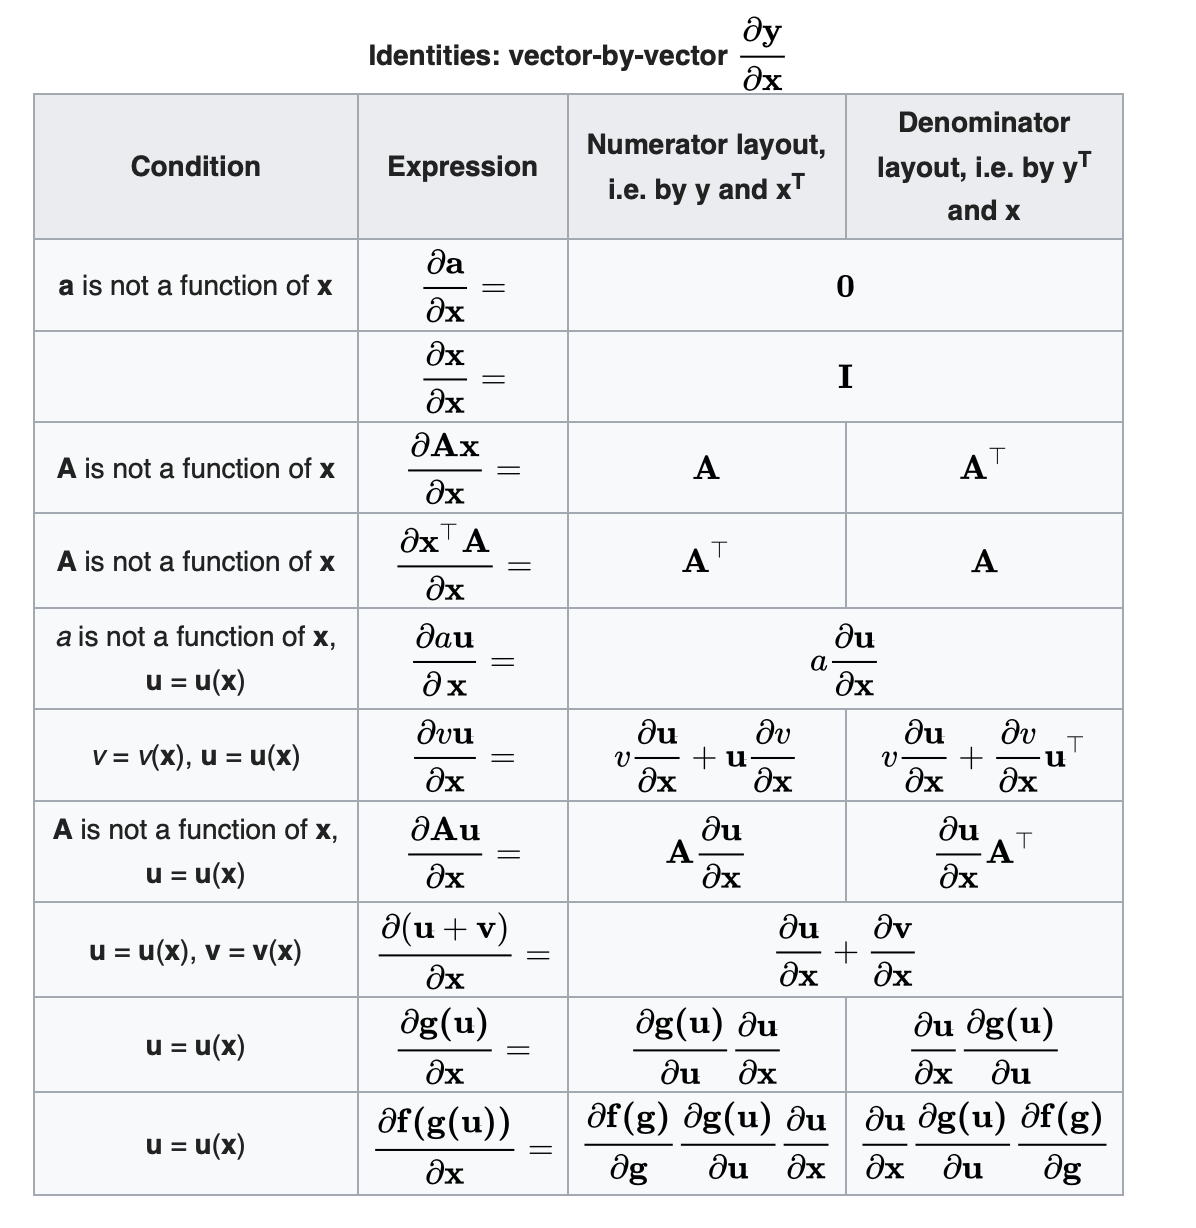
\includegraphics[scale=0.25]{vector_by_vector.png}
    \caption{Denominator layout means $x\in\mathbb{R}^{n\times 1}$}
    \label{}
\end{figure}\end{center}

\begin{equation}
    \begin{aligned}
        \frac{\partial u}{\partial x^T}&=(\frac{\partial u^T}{\partial x})^T\\
        \frac{\partial u^Tv}{\partial x}&=\frac{\partial u^T}{\partial x}v+\frac{\partial v^T}{\partial x}u^T\\
        \frac{\partial uv^T}{\partial x}&=\frac{\partial u}{\partial x}v^T+u\frac{\partial v^T}{\partial x}\\
        \frac{\partial x^Tx}{\partial x}&=2x\\
        \frac{\partial x^TAx}{\partial x}&=(A+A^T)x\\
    \end{aligned}
    \nonumber
\end{equation}
where $x,u,v\in \mathbb{R}^{n\times 1}$

$\textbf{Note:}$ $$\frac{d\|Aw-b\|^2}{dw}
=\frac{d(Aw-b)^T(Aw-b)}{dw}
\\=\frac{d(Aw-b)^T}{dw}(Aw-b)+\frac{d(Aw-b)^T}{dw}(Aw-b)
\\=2A^T(Aw-b)$$

Matrix by vector:
\begin{equation}
    \begin{aligned}
        \frac{\partial AB}{\partial x}&=\frac{\partial A}{\partial x}B+A\frac{\partial B}{\partial x}
    \end{aligned}
    \nonumber
\end{equation}

Matrix by matrix:
\begin{equation}
    \begin{aligned}
        \frac{\partial u^TXv}{\partial X}&=uv^T\\
        \frac{\partial u^TX^TXu}{\partial X}&=2Xuu^T\\
        \frac{\partial [(Xu-v)^T(Xu-v)]}{\partial X}&=2(Xu-v)u^T\\
    \end{aligned}
    \nonumber
\end{equation}

Trace:
\begin{equation}
    \begin{aligned}
        tr(a)&=a\\
        tr(AB)&=tr(BA)\\
        tr(ABC)=&tr(CAB)=tr(BCA)\\
        \frac{\partial tr(AB)}{\partial A}&=B^T\\
        tr(A)&=tr(A^T)\\
        \frac{\partial tr(ABA^TC)}{\partial A}&=CAB+C^TAB^T
    \end{aligned}
    \nonumber
\end{equation}

\section{Matrix Inversion}
\subsection{Woodbury matrix identity}
$${\displaystyle \left(A+UCV\right)^{-1}=A^{-1}-A^{-1}U\left(C^{-1}+VA^{-1}U\right)^{-1}VA^{-1},}$$
where $A, U, C$ and $V$ are conformable matrices: $A$ is $n\times n$, $C$ is $k\times k$, $U$ is $n\times k$, and $V$ is $k\times n$. This can be derived using blockwise matrix inversion.

\underline{Blockwise inversion: }$$
{\displaystyle {\begin{bmatrix}\mathbf {A} &\mathbf {B} \\\mathbf {C} &\mathbf {D} \end{bmatrix}}^{-1}={\begin{bmatrix}\mathbf {A} ^{-1}+\mathbf {A} ^{-1}\mathbf {B} \left(\mathbf {D} -\mathbf {CA} ^{-1}\mathbf {B} \right)^{-1}\mathbf {CA} ^{-1}&-\mathbf {A} ^{-1}\mathbf {B} \left(\mathbf {D} -\mathbf {CA} ^{-1}\mathbf {B} \right)^{-1}\\-\left(\mathbf {D} -\mathbf {CA} ^{-1}\mathbf {B} \right)^{-1}\mathbf {CA} ^{-1}&\left(\mathbf {D} -\mathbf {CA} ^{-1}\mathbf {B} \right)^{-1}\end{bmatrix}}}
$$







\section{Linear Regression: Least Square}
$\textbf{Minimize}_w \mathcal{R}(w)=\|Xw-y\|^2$
\subsection{Normal Equations}
$$\nabla_w\|Xw-y\|^2=2X^T(Xw-y)=0$$
$$\Rightarrow X^TXw=X^Ty$$
These are called the \textbf{normal equations}.
\begin{proposition}
    $\hat{w}$ satisfies $\mathcal{R}(\hat{w})=\min_w\mathcal{R}(w)$ if and only if $\hat{w}$ satisfies the normal equations. (i.e. prove its is the global minimum)
\end{proposition}
\begin{proof}
Consider $\boldsymbol{w}$ with $\boldsymbol{X}^{\top} \boldsymbol{X} \boldsymbol{w}=\boldsymbol{X}^{\top} \boldsymbol{y}$, and any $\boldsymbol{w}^{\prime}$; then $$\begin{aligned}\left\|\boldsymbol{X} \boldsymbol{w}^{\prime}-\boldsymbol{y}\right\|^{2} &=\left\|\boldsymbol{X} \boldsymbol{w}^{\prime}-\boldsymbol{X} \boldsymbol{w}+\boldsymbol{X} \boldsymbol{w}-\boldsymbol{y}\right\|^{2} \\ &=\left\|\boldsymbol{X} \boldsymbol{w}^{\prime}-\boldsymbol{X} \boldsymbol{w}\right\|^{2}+2\left(\boldsymbol{X} \boldsymbol{w}^{\prime}-\boldsymbol{X} \boldsymbol{w}\right)^{\top}(\boldsymbol{X} \boldsymbol{w}-\boldsymbol{y})+\|\boldsymbol{X} \boldsymbol{w}-\boldsymbol{y}\|^{2} \end{aligned}$$
Since
$$
\left(\boldsymbol{X} \boldsymbol{w}^{\prime}-\boldsymbol{X} \boldsymbol{w}\right)^{\top}(\boldsymbol{X} \boldsymbol{w}-\boldsymbol{y})=\left(\boldsymbol{w}^{\prime}-\boldsymbol{w}\right)^{\top}\left(\boldsymbol{X}^{\top} \boldsymbol{X} \boldsymbol{w}-\boldsymbol{X}^{\top} \boldsymbol{y}\right)=0
$$
then
$$
\left\|\boldsymbol{X} \boldsymbol{w}^{\prime}-\boldsymbol{y}\right\|^{2}=\left\|\boldsymbol{X} \boldsymbol{w}^{\prime}-\boldsymbol{X} \boldsymbol{w}\right\|^{2}+\|\boldsymbol{X} \boldsymbol{w}-\boldsymbol{y}\|^{2} \geq\|\boldsymbol{X} \boldsymbol{w}-\boldsymbol{y}\|^{2}
$$
\end{proof}

\section{LU Decomposition (Restricted to Square)}
Triangular matrix saves time when computing $Ax=b$.

Let A be a square matrix. An LU factorization refers to the factorization of A, with proper row and/or column orderings or permutations, into two factors - a lower triangular matrix L and an upper triangular matrix U:

${\displaystyle A=LU.}$
In the lower triangular matrix all elements above the diagonal are zero, in the upper triangular matrix, all the elements below the diagonal are zero. For example, for a $3 \times 3$ matrix $A$, its LU decomposition looks like this:

$${\displaystyle {\begin{bmatrix}a_{11}&a_{12}&a_{13}\\a_{21}&a_{22}&a_{23}\\a_{31}&a_{32}&a_{33}\end{bmatrix}}={\begin{bmatrix}\ell _{11}&0&0\\\ell _{21}&\ell _{22}&0\\\ell _{31}&\ell _{32}&\ell _{33}\end{bmatrix}}{\begin{bmatrix}u_{11}&u_{12}&u_{13}\\0&u_{22}&u_{23}\\0&0&u_{33}\end{bmatrix}}.}$$

$$A=PLU$$
$P$ is a permutation matrix (used to swap row, only one $1$ in every row). $P$ is orthogonal, so $P^{-1}=P^T$.

Solve $Ax=b$:
\begin{equation}
    \begin{aligned}
        Ax&=b\\
        PLUx&=b\\
        \text{Let }y=Ux,&\text{ then solve PLy=b}\\
        Ly&=P^Tb
    \end{aligned}
    \nonumber
\end{equation}
Complexity: $O(n^3)$

\section{SVD: Singular Value Decomposition}
For a $n\times m$ matrix $A$ with rank $r$,
\begin{equation}
    \begin{aligned}
        A_{n\times m}=&U_{n\times n}\Sigma_{n\times m}V^T_{m\times m}\\
        &=\sum_{i=1}^rs_iu_iv_i^T\\
        &=\begin{bmatrix}
            \vline&\vline&\cdots&\vline\\
            u_1&u_2&\cdots&u_n\\
            \vline&\vline&\cdots&\vline
        \end{bmatrix}\begin{bmatrix}
            s_1&&&&&&\\
            &s_2&&&&&\\
            &&\ddots&&&&\\
            &&&s_r&&&\\
            &&&&0&&\\
            &&&&&\ddots&\\
            &&&&&&0
        \end{bmatrix}\begin{bmatrix}
            \vline&\vline&\cdots&\vline\\
            v_1&v_2&\cdots&v_m\\
            \vline&\vline&\cdots&\vline
        \end{bmatrix}^T
    \end{aligned}
    \nonumber
\end{equation}
$U,V$ are orthogonal matrices. $u_i\in \mathbb{R}^{n\times 1}$ are left singular vectors, $v_i\in \mathbb{R}^{m\times 1}$ are right singular vectors. $s_i,i=1,...,r$ are singular values (absolute values of eigenvalues of a normal matrix).

Complexity:$O(mn^2+n^3)$


\subsection{Pseudo-inverse}
We can't compute the inverse matrix of a singular matrix. We can use pseudo-inverse matrix.
$$A^+_{m\times n}=\sum_{i=1}^r\frac{1}{s_i}v_iu_i^T=V\Sigma^+U^T$$
Where $$\Sigma^+=\begin{bmatrix}
    \frac{1}{s_1}&&&&&&\\
    &\frac{1}{s_2}&&&&&\\
    &&\ddots&&&&\\
    &&&\frac{1}{s_r}&&&\\
    &&&&0&&\\
    &&&&&\ddots&\\
    &&&&&&0
\end{bmatrix}$$
The SVD may not be unique, but the pseudo-inverse of $A$, $A^+$ is unique.
\begin{equation}
    \begin{aligned}
        AA^+&=\sum_{i=1}^ru_iu_i^T=\begin{bmatrix}
            I_{r\times r}&	O_{r\times n-r}\\
            O_{n-r\times r}&	O_{n-r\times n-r}
        \end{bmatrix}_{n\times n}\\
        A^+A&=\sum_{i=1}^rv_iv_i^T=\begin{bmatrix}
            I_{r\times r}&	O_{r\times m-r}\\
            O_{m-r\times r}&	O_{m-r\times m-r}
        \end{bmatrix}_{m\times m}
    \end{aligned}
    \nonumber
\end{equation}
If $A^{-1}$ exists, $A^{-1}=A^+$.

\subsection{Analysis of $A^TA$ and $AA^T$}
\begin{equation}
    \begin{aligned}
        A^TA&=(U\Sigma V^T)^T(U\Sigma V^T)\\
        &=V\Sigma^TU^TU\Sigma V^T\\
        &=V\Sigma^T\Sigma V^T\\
        &=V\Sigma^2 V^T\\
        \Rightarrow	V&=A^TU\Sigma^+
    \end{aligned}
    \nonumber
\end{equation}
Columns of $V$ are the eigenvectors of $A^TA$.

The diagonal entries of $\Sigma^2$, $s_1^2,s_2^2,...,s_r^2$ are the eigenvalues of $A^TA$.

Similarly: $$AA^T=U\Sigma^2U^T$$
$$\Rightarrow U=AV\Sigma^+$$
Columns of $U$ are the eigenvectors of $AA^T$.

\textbf{Fact:} $A^TA$ is positive semi-definite.

\subsection{Solve Normal Equations}
Solve $X^TXw=X^Ty$, $$\hat{w}_{ols}=X^+y$$
$$X^TX\hat{w}_{ols}=X^TXX^+y=(X^T(XX^+))y=X^Ty$$

\subsection{Low-Rank Approximation}
For a $n\times m$ matrix $A$ with rank $r$, $A=\sum_{i=1}^rs_iu_iv_u^T$.

\textbf{Rank-$k$ approximation} for $A$ is
$$A_k=\sum_{i=1}^ks_iu_iv_u^T$$
Where $s_1\geq s_2\geq \cdots\geq 0$




\begin{thebibliography}{1}
    \bibitem{Long2015Fully}  MATH 417: Christopher J Leininger  \newblock Introduction to Abstract Algebra (Draft)  2017.
    \bibitem{Long2015Fully} MATH 484
    \bibitem{Long2015Fully} ECE 490
    \bibitem{Long2015Fully} STAT 425
    \bibitem{Long2015Fully} CS/MATH 357
\end{thebibliography}


\end{document}
\bibliography{reference}
\bibliographystyle{unsrt}